\documentclass{article}

\usepackage{graphicx}
\usepackage[margin=2cm]{geometry}
\usepackage{verbatim}
\usepackage[export]{adjustbox}

\begin{document}

\newcommand{\modefont}[1]{\texttt{#1}}
\newcommand{\mnocheck}{\modefont{nocheck}}
\newcommand{\mnonstrict}{\modefont{nonstrict}}
\newcommand{\mstrict}{\modefont{strict}}

%% ---
\subsection*{Figure 3: Records per Hour}

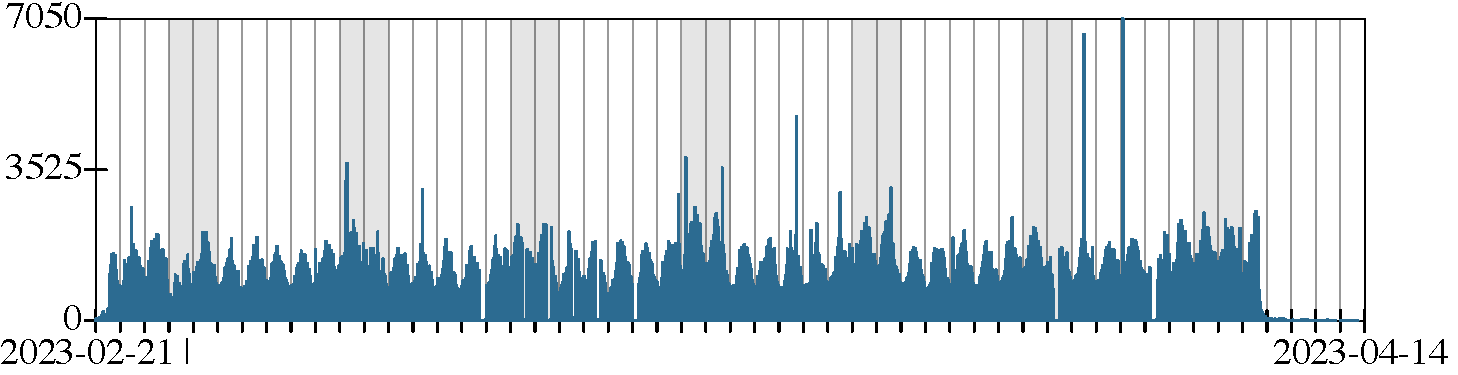
\includegraphics[width=\columnwidth]{out/row-distribution.pdf}

TODO reason for sending


%% ---
\subsection*{Table 2: Size of Analyzed Code}

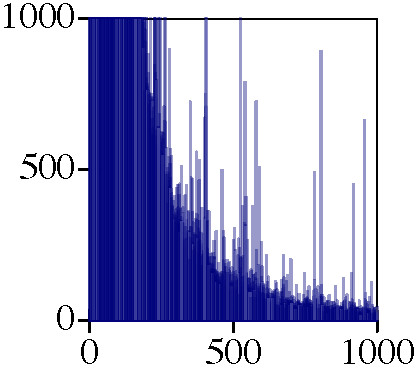
\includegraphics[width=0.4\columnwidth]{out/lines-distribution.pdf}
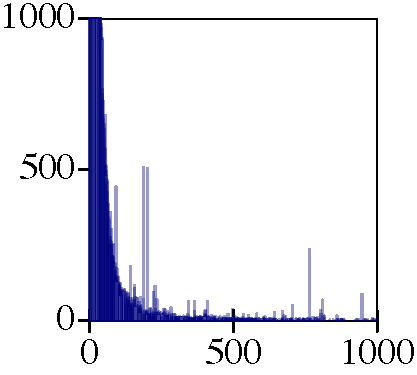
\includegraphics[width=0.4\columnwidth]{out/editrange-distribution.pdf}

TODO mean stddev median P99


%% ---
\subsection*{Table 3: Session Size}

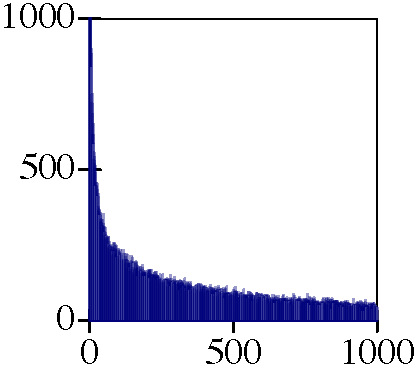
\includegraphics[width=0.4\columnwidth]{out/timespan-distribution.pdf}
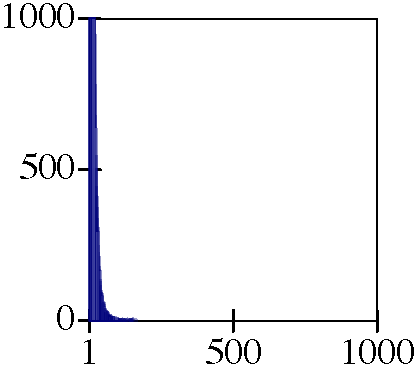
\includegraphics[width=0.4\columnwidth]{out/event-count-distribution.pdf}

TODO mean stddev median P99


%% ---
\subsection*{Table 4: Current Type Errors and Background Errors}

TODO


%% ---
\subsection*{Figure 4: Overview of Mode Usage}

TODO


%% ---
\subsection*{Figure 5: Type and Background Errors Grouped by Mode}

{ \newcommand{\labelbars}[1]{\begin{tabular}[t]{l@{}l} \raisebox{2ex}{\begin{tabular}[t]{r}\mnocheck{}\\\mnonstrict{}\\\mstrict{}\end{tabular}} & #1 \end{tabular}}
  \begin{tabular}[t]{cc}
    Type errors & Background errors \\
    \labelbars{\includegraphics[width=0.20\columnwidth,valign=M]{out/error-by-mode-te.pdf}}
    & \labelbars{\includegraphics[width=0.20\columnwidth,valign=M]{out/error-by-mode-fs.pdf}}
  \end{tabular}
}


%% ---
\subsection*{Table 5: Specific Errors in Edit Range}

TODO


%% ---
\subsection*{Table 6: Type Error Popularity}

TODO

{\footnotesize
\verbatiminput{out/ctc-info.txt}
}


%% ---
\subsection*{Figure 6: Type Error Density}

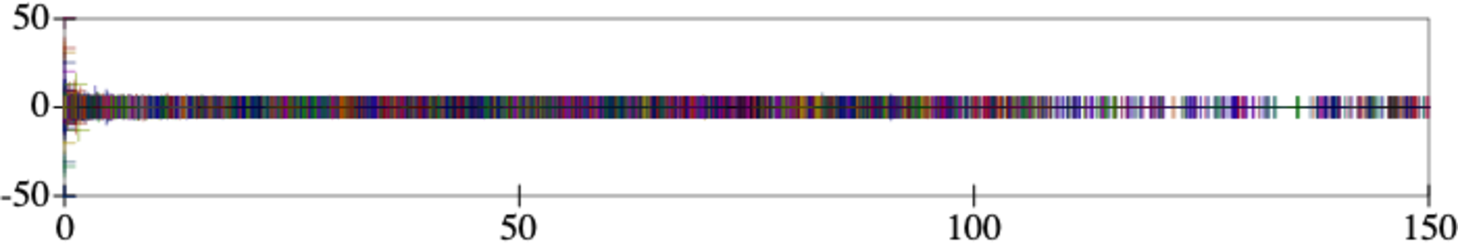
\includegraphics[width=\columnwidth]{out/error-count-nocheck-row--te-density-diff.pdf}
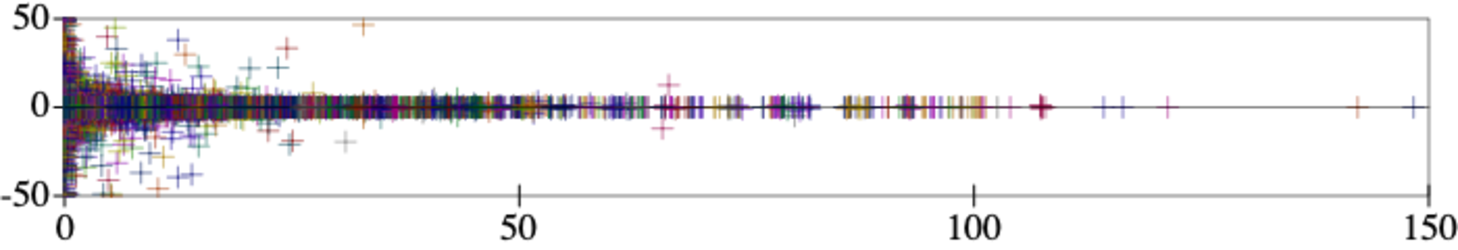
\includegraphics[width=\columnwidth]{out/error-count-nonstrict-row--te-density-diff.pdf}
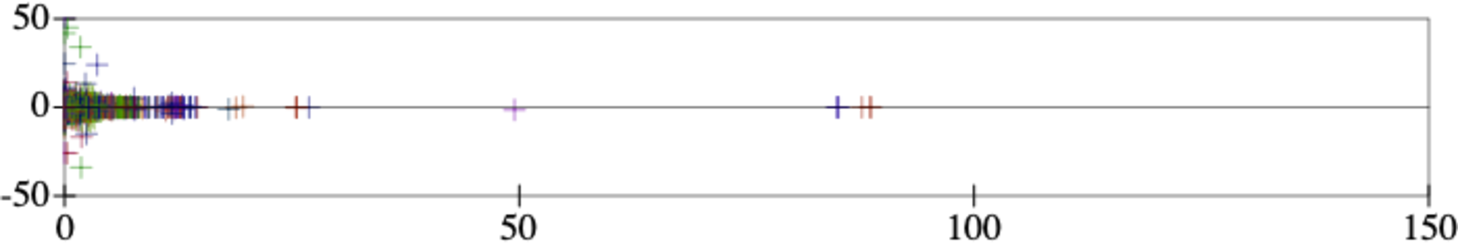
\includegraphics[width=\columnwidth]{out/error-count-strict-row--te-density-diff.pdf}


\end{document}
